\chapter{Determinism} 
\label{jitterDeterminismNetworkDimention}

An Ethernet frames sent by various sources (e.g.: WR Node) will reach their
destinations with different delays. A packet's delay varies with:
\begin{itemize}
  \item the source's position in the network,
  \item the numbers of hops along the path,
  \item load of traffic ,
  \item Class of Service, priority.
\end{itemize}
This variation in delay is known as jitter. Determinism of packets' delivery in
Ethernet network is understood in this document as predictability of its delay.
A deterministic network is the one in which the delay of packet's delivery from
the source to the receiver is guaranteed to be within a set time. This time is
called \GranularityWindow (\GW). 

Carefully configured and properly used White Rabbit Network offers
deterministic Ethernet Frame delivery for routed unicast and broadcast traffic
\footnote{It is true, if the \HP\ Bypass described in
Chapter~\ref{chapter:HPbypass} is not enabled.}
(Appendix~\ref{appH} details estimation of Ethernet Frame delivery delay). This
is possible thanks to the implementation of Class of Service (CoS) and the fact
that the delay introduced by the switch can be verified by analysis of publicly
available source code. By routed traffic, we understand store-and-forward
traffic whose destination is determined by Routing Table Unit (RTU) and which is
stored and forwarded using Switching Core (Swcore). Figure~\ref{fig:swRouting}
gives an overview of the routing mechanism in WR Switch, details of WR Switch
routing implementation are available in the
presentation \cite{HWpresentation}.




In White Rabbit Network the requirements regarding determinism are
straightforward: \ControlMessage\ (which is transported by a number of Ethernet
Frames) shall traverse from Data Master to all Nodes within a \GW\ of 100$\mu$
for GSI and 1000$ \mu$ for CERN. In this chapter, we introduce a mechanism used
to decrease delivery delay of critical data and explain it's WR-specific usage.
We present estimation of a \ControlMessage\ delivery delay for an existing
implementation of WR Switches and suggest improvements to help achieve the
demanding requirements.

\begin{center}
	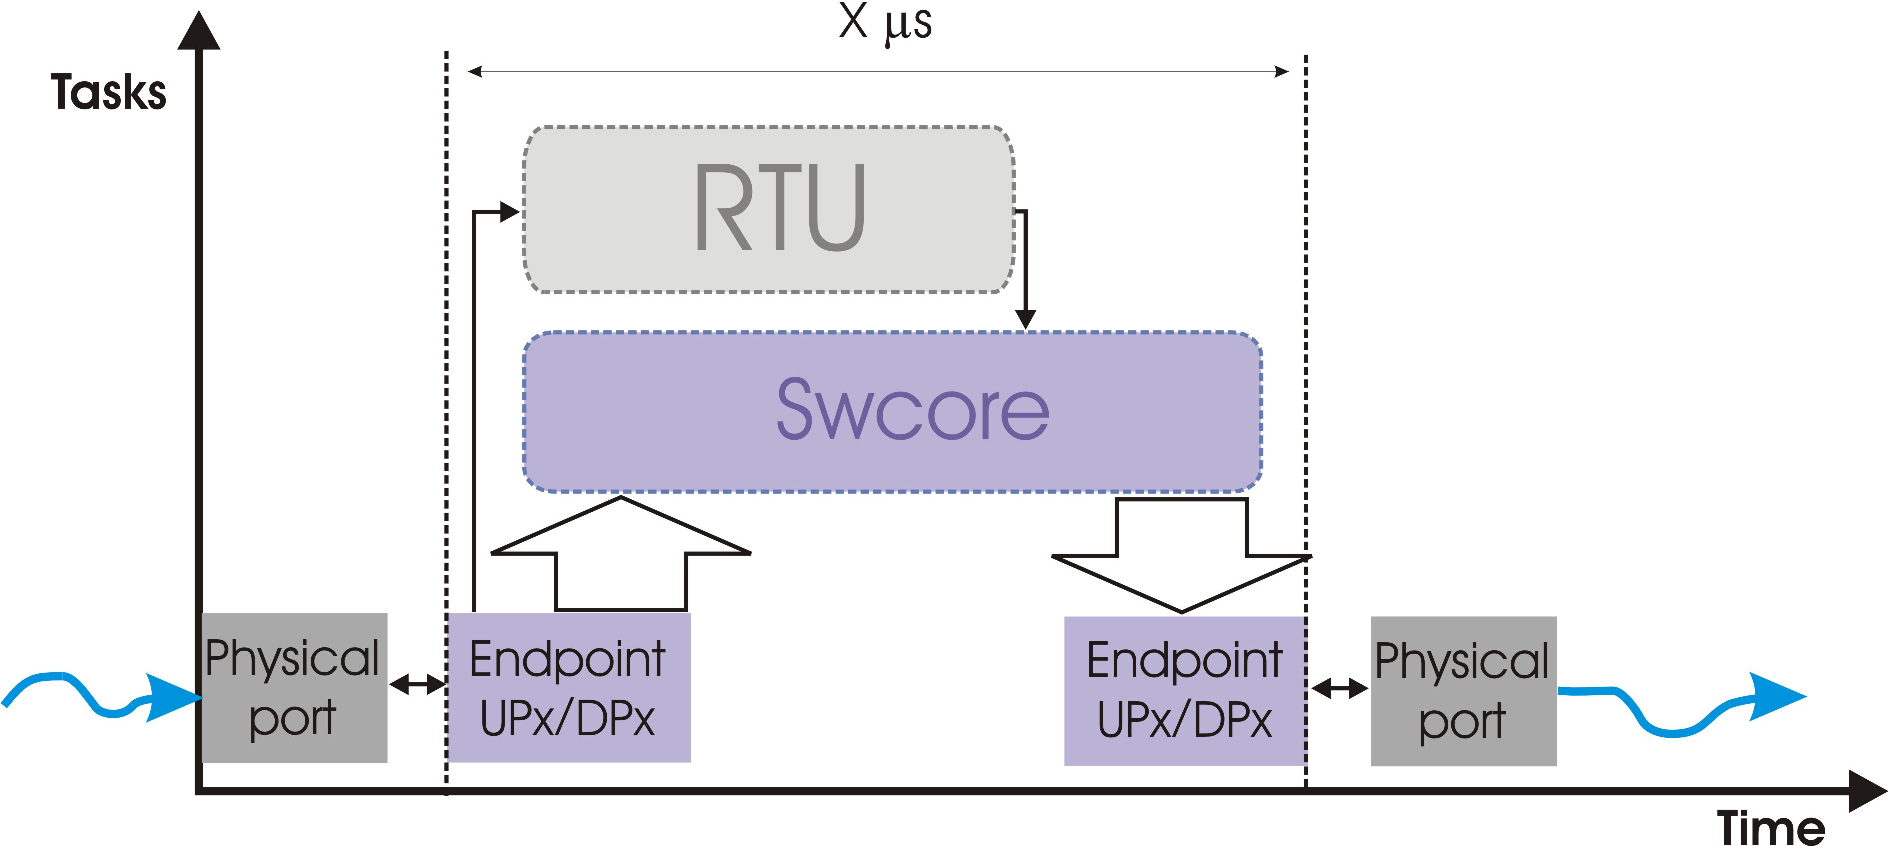
\includegraphics[scale=0.30]{robustness/switchRouting.ps}
	\captionof{figure}{WR Switch routing using Swcore and RTU (not to
			  scale).}
	\label{fig:swRouting}
\end{center}

%%%%%%%%%%%%%%%%%%%%%%%%%%%%%%%%%%%%%
\section{CoS and Traffic Prioritize}
\label{chapter:cos}
%%%%%%%%%%%%%%%%%%%%%%%%%%%%%%%%%%%%%

Class of Service defines (CoS) different levels of priority. The network
provides higher levels of service to those applications operating at higher
priorities, but no explicit guarantees are made. The highest priority
class will get the best available service, but the priorities are assigned to
each frame on a frame-by-frame basis. There are eight different classes of
service, as expressed through the 3-bit PCP field in the header added to the
frame ~\ref{fig:VLAN_Tag}, defined in the standard \cite{IEEE8021Q}.


The association of certain type of traffic to one of CoS levels can be defined
by configuration and issued by the sender node. The switch provides the best
available service by putting the higher-priority frames in the queue associated
with the higher CoS, but there is no guarantee that this will meet any specified
minimum level. The same applies to the rest of CoS. 

\begin{figure}[!ht]
 \centering
		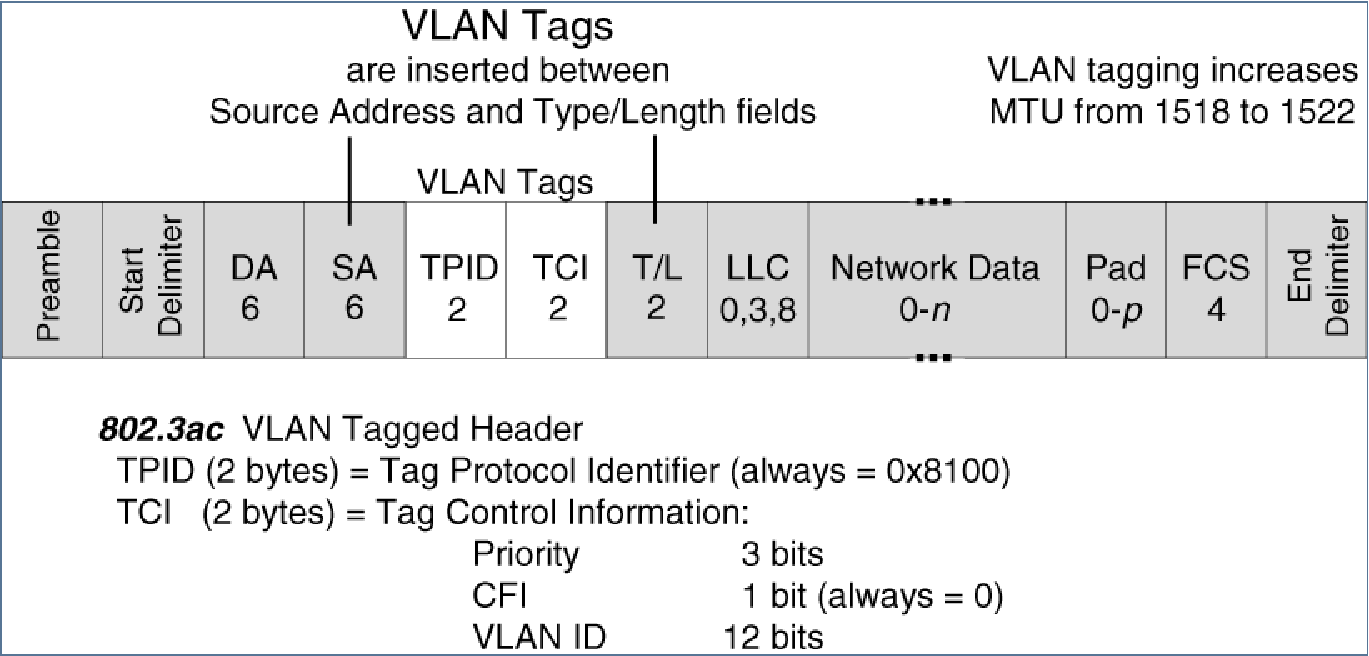
\includegraphics[scale=0.30]{robustness/VLAN_Tag_GigaPeek.ps}
 \caption{VLAN Tags}
	\label{fig:VLAN_Tag}
\end{figure}


White Rabbit Switch implements the 8 priorities defined by the \cite{IEEE8021Q}.
According to the standard, the usage of a broadcast/unicast destination address
does make no difference regarding the priority of traffic. However, in WR the
highest priority is broken down two-fold, so as to differentiate between the
frames of \ControlMessage, broadcast, and traffic tagged with highest priority
without control information which is unicast. This condition
is created for the sake of jitter during the routing in the
switches as explained in the Chapter ~\ref{HPbypass}. By doing this, WR CoS can
provide to the highest priority broadcast traffic, the resources to
achieve the required upper bound of latency and guarantee maximum throughput.
Thus, we'll distinguish between:

\begin{itemize}
	\item \HP, defined upper bound of latency and maximum throughput.
	\item \SP, non-defined upper bound of latency.
\end{itemize}

Since WR CoS introduces an address-based condition for distinguishing between
\HP\ and \SP, the following default/recommended addressing conditions and WR
role shall be consider by the user:

\begin{itemize}
	\item Only the Data Master WR Node shall send frames with 7th priority
	      and broadcast address \footnote{Sending of frames with 7th
	      priority and broadcast by non-Data Master WR Nodes is foreseen,
	      read the chapter~\ref{chap:deter_control_message} for details}.
	      This frames shall contain \ControlMessage s.
	\item Only the frames tagged with 7th priority and
	      broadcast are guaranteed to have upper bound latency while
	      routing. The other frames, including 7th priority unicast, does
	      not offer upper bound latency.
	\item If a WR Node (non-Data Master) wants to send a broadcast frame, it
	      can only do it using 7th priority unicast and 6th - 0th priority	
	      \footnote{Applies to recommented configuration.}.
\end{itemize}


 
A non-default configuration, e.g.: with a few Active Data Master Nodes, is
possible but might deteriorate reliability and determinism of the system.


\begin{table}[!ht]
\begin{center}
\begin{tabular}{|c|c|c|c|}
\hline
\textbf{PCP} & \textbf{Network Priority} & \textbf{WR Conf. default} &
\textbf{Addressing Scheme} \\ \hline
1 & 0 (lowest) &  Protocols Traffic & Broadcast/Unicast \\  \hline
0 & 1 & Standard Data & Broadcast/Unicast  \\  \hline
2 & 2 &  user defined & Broadcast/Unicast \\  \hline
3 & 3 & user defined & Broadcast/Unicast \\  \hline
4 & 4 & user defined & Broadcast/Unicast \\  \hline
5 & 5 &  user defined& Broadcast/Unicast \\  \hline
6 & 6 & user defined & Broadcast/Unicast \\  \hline
7 & 7u & Control Data & Unicast  \\  \hline
7 & 7b (Highest) & Control Data & Broadcast \\  \hline
\end{tabular}
\caption{Class of Service and Addressing in WR}
\label{tab:CoS}
\end{center}
\end{table}


%%%%%%%%%%%%%%%%%%%%%%%%%%%%%%%%%%%%%%%%%
\section{Determinism of Control Messages}
\label{chap:deter_control_message}
%%%%%%%%%%%%%%%%%%%%%%%%%%%%%%%%%%%%%%%%%


In Deterministic Control Systems the execution of the \ControlMessage\ by the
receivers is tied up to \GranularityWindow (\GW). \ControlMessage's size is
assumed to be fixed (for a given system/configuration). We will consider three
possible sizes of \ControlMessage s which fit into GSI's and CERN's
requirements: 500bytes, 1500bytes and 5000bytes. Since a \ControlMessage\ is
encoded into a number of Ethernet Frames \footnote{It is forced by the FEC
encoding described in Chapter~\ref{chapter:FEC}}, the estimation of
\ControlMessage\ Delivery Delay will differ from Ethernet Frame Delivery Delay
(described in Appendix~\ref{appH}). The following facts need to be taken into
account when estimating Delivery Delay of a \ControlMessage:
\begin{itemize}
  \item We need to calculate deliver of a few Ethernet frames in a burst,
approx.: 4.
  \item The size of a single Ethernet frames is different from \ControlMessage\
size, see Table~\ref{tab:FECedSize}.
  \item Encoding and decoding (e.g.: FEC) needs to be included into
calculations.
\end{itemize}


\begin{table}[ht]
\caption{Transmission times of FECed \ControlMessage s.} 
\centering
	\begin{tabular}{| p{2.5cm} | p{2.5cm} | p{2.5cm} | p{4cm} |}  \hline
\textbf{\ControlMessage\ size}&\textbf{FECed \HP\ Package size} &\textbf{Number
of \HP\ Packages}& \textbf{Transmission Time of \HP\ Package}\\ \hline
500 bytes  & 375 bytes       & 4   & 3$\mu s$      \\ \hline
1500 bytes & 1125 bytes      & 4   & 9$\mu s$      \\ \hline
5000 bytes & 1454 bytes      & 8   & 12$\mu s$      \\ \hline

\end{tabular}
\label{tab:FECedSize}
\end{table}

\begin{center}
	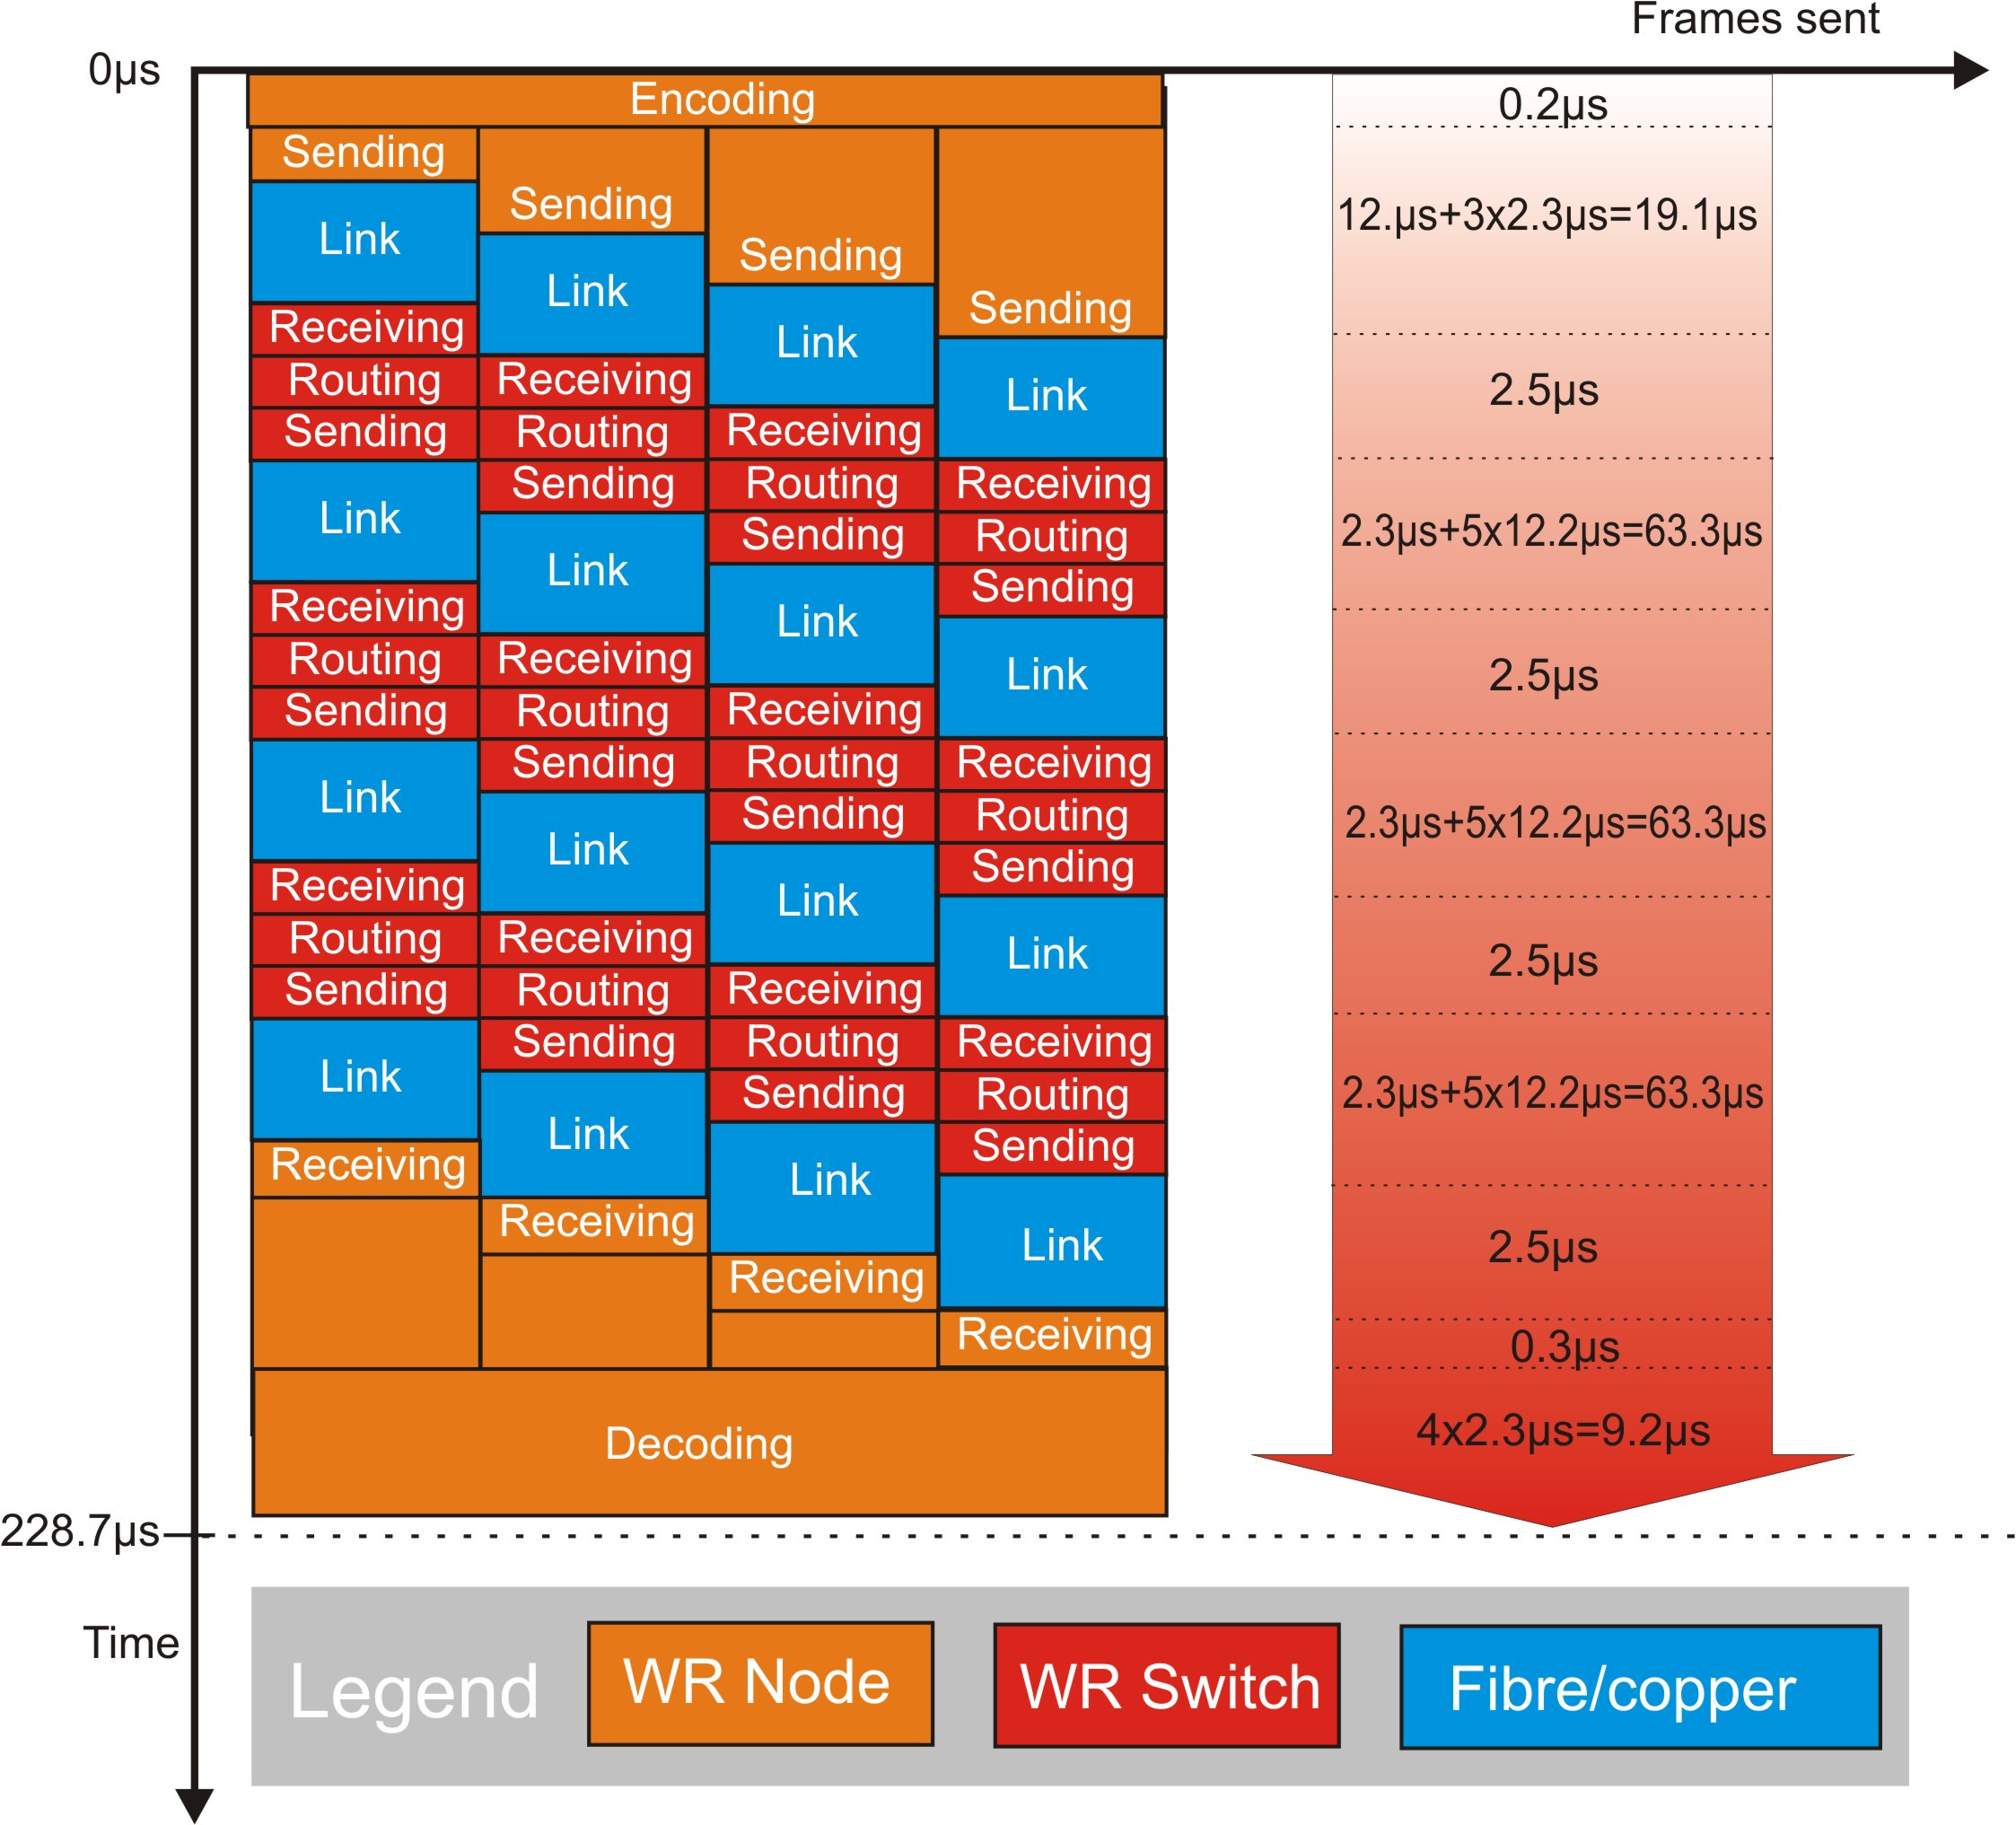
\includegraphics[scale=0.35]{robustness/CMdelayStandard.ps}
	\captionof{figure}{Delivery Delay of \ControlMessage\ (not to scale),
for description how the numbers were obtained, see Appendix~\ref{appH}.}
	\label{fig:CMdelayStandard}
\end{center}

Figure~\ref{fig:CMdelayStandard} depicts estimation of \ControlMessage\ Delivery
Delay \footnote{The time of 1500byte Ethernet Frame reception is $12.176\mu s$,
in the calculations, it is overestimated to $13\mu s$.}   encoded into 4
Ethernet frame (see Table~\ref{tab:EtherFrameDelayGeneral} and 
Appendix~\ref{appH} for detailed descriptions). The estimation makes the
following assumptions:
\begin{itemize}
  \item \ControlMessage\ size is 500 bytes.
  \item \ControlMessage\ is encoded by FEC into 4 Ethernet Frames of 375 bytes
each.
  \item We assume the parameter $B$ to be 0 for the node (see
Table~\ref{tab:EtherFrameDelayGeneral} and Appendix~\ref{appH}).
  \item We assume parameter $B$ to be 5 for the switch (see
Table~\ref{tab:EtherFrameDelayGeneral} and Appendix~\ref{appH}).
  \item The total length of the links is 2km, GSI use case.
\end{itemize}

\begin{table}[ht]
\caption{Elements of Ethernet frame delivery delay estimation.} 
\centering
	\begin{tabular}{| l |  c | c | c |}          \hline
\textbf{Name}&\textbf{Symbol}&\textbf{Value}&\textbf{Value}                  \\
                                 &                &  Min& Max          \\ \hline
% Sending node
Ethernet Frame Transmission Delay&$delay_{n\_tx}$&$0\mu s$&$(13 + B * 13)\mu s$
\\ \hline
% Switch
Switch Routing Delay &$delay_{n\_sw}$&$13\mu s$ &$(13 + B * 13)\mu s$ 
 
\\ \hline
% Links
Link Delay                       & $delay_{link}$ &5 [$\frac{\mu
s}{km}$]&5 [$\frac{\mu s}{km}$]      
\\ \hline
% Receivning node
Ethernet Frame Reception delay   & $delay_{n\_rx}$&$13\mu s$&$13\mu s$

\\ \hline
\end{tabular}
\label{tab:EtherFrameDelayGeneral}
\end{table}


Different Use Cases estimations of \ControlMessage\ Delivery Delay for GSI (2km)
and CERN (10km) are included in Table~\ref{tab:CMspDelay}.

\begin{table}[ht]
\caption{\ControlMessage\ Deliver Delay.} 
\centering
	\begin{tabular}{| c | c | c | c |}          \hline
\textbf{\ControlMessage\ size}& \multicolumn{2}{|c|}{\textbf{\ControlMessage\
Delivery Delay}}\\
               &    GSI           & CERN          \\ \hline
500 bytes      & 221$\mu s$       & 283$\mu s$    \\ \hline
1500 bytes     & 285$\mu s$       & 325$\mu s$    \\ \hline
5000 bytes     & 324$\mu s$       & 364$\mu s$    \\ \hline
\end{tabular}
\label{tab:CMspDelay}
\end{table}
%%%%%%%%%%%%%%%%%%%%%%%%%%%%%%%%%%%
\section{\HighPriority Bypass}
\label{chapter:HPbypass}
%%%%%%%%%%%%%%%%%%%%%%%%%%%%%%%%%%%


The following conclusions can be derived from the estimations in the previous
sections:
\begin{itemize}
  \item GSI's requirements are not fulfilled.
  \item The jitter is very big.
\end{itemize}

It has to be noticed that the GSI's requirements apply only to Control Messages
which are always broadcast at the highest level of CoS. This fact is very
important and enables to propose a solution to above-mentioned problems 
(limitations). The broadcast Ethernet frames do not need routing according to
MAC address which is provided by RTU. In order to be standard compatible,
broadcast traffic needs to be routed by VLANs though. This process is definitely
easier and can be done on-the-fly. As a consequence, it has been proposed to
distinguish broadcast 7 (highest priority) level of CoS traffic from the rest
of the Ethernet traffic. It is called in this document \HighPriority\ Traffic
(\HP\ Traffic) and the Ethernet frames of such traffic are called \HighPriority\
Packages (\HP\ Packages). On the contrary, non-\HP Traffic, is called in this
document \StandardPriority\ Traffic (\SP\ Traffic) and non-\HP\ Packages are
called
\StandardPriority\ Packages (\SP\ Packages).

\begin{center}
	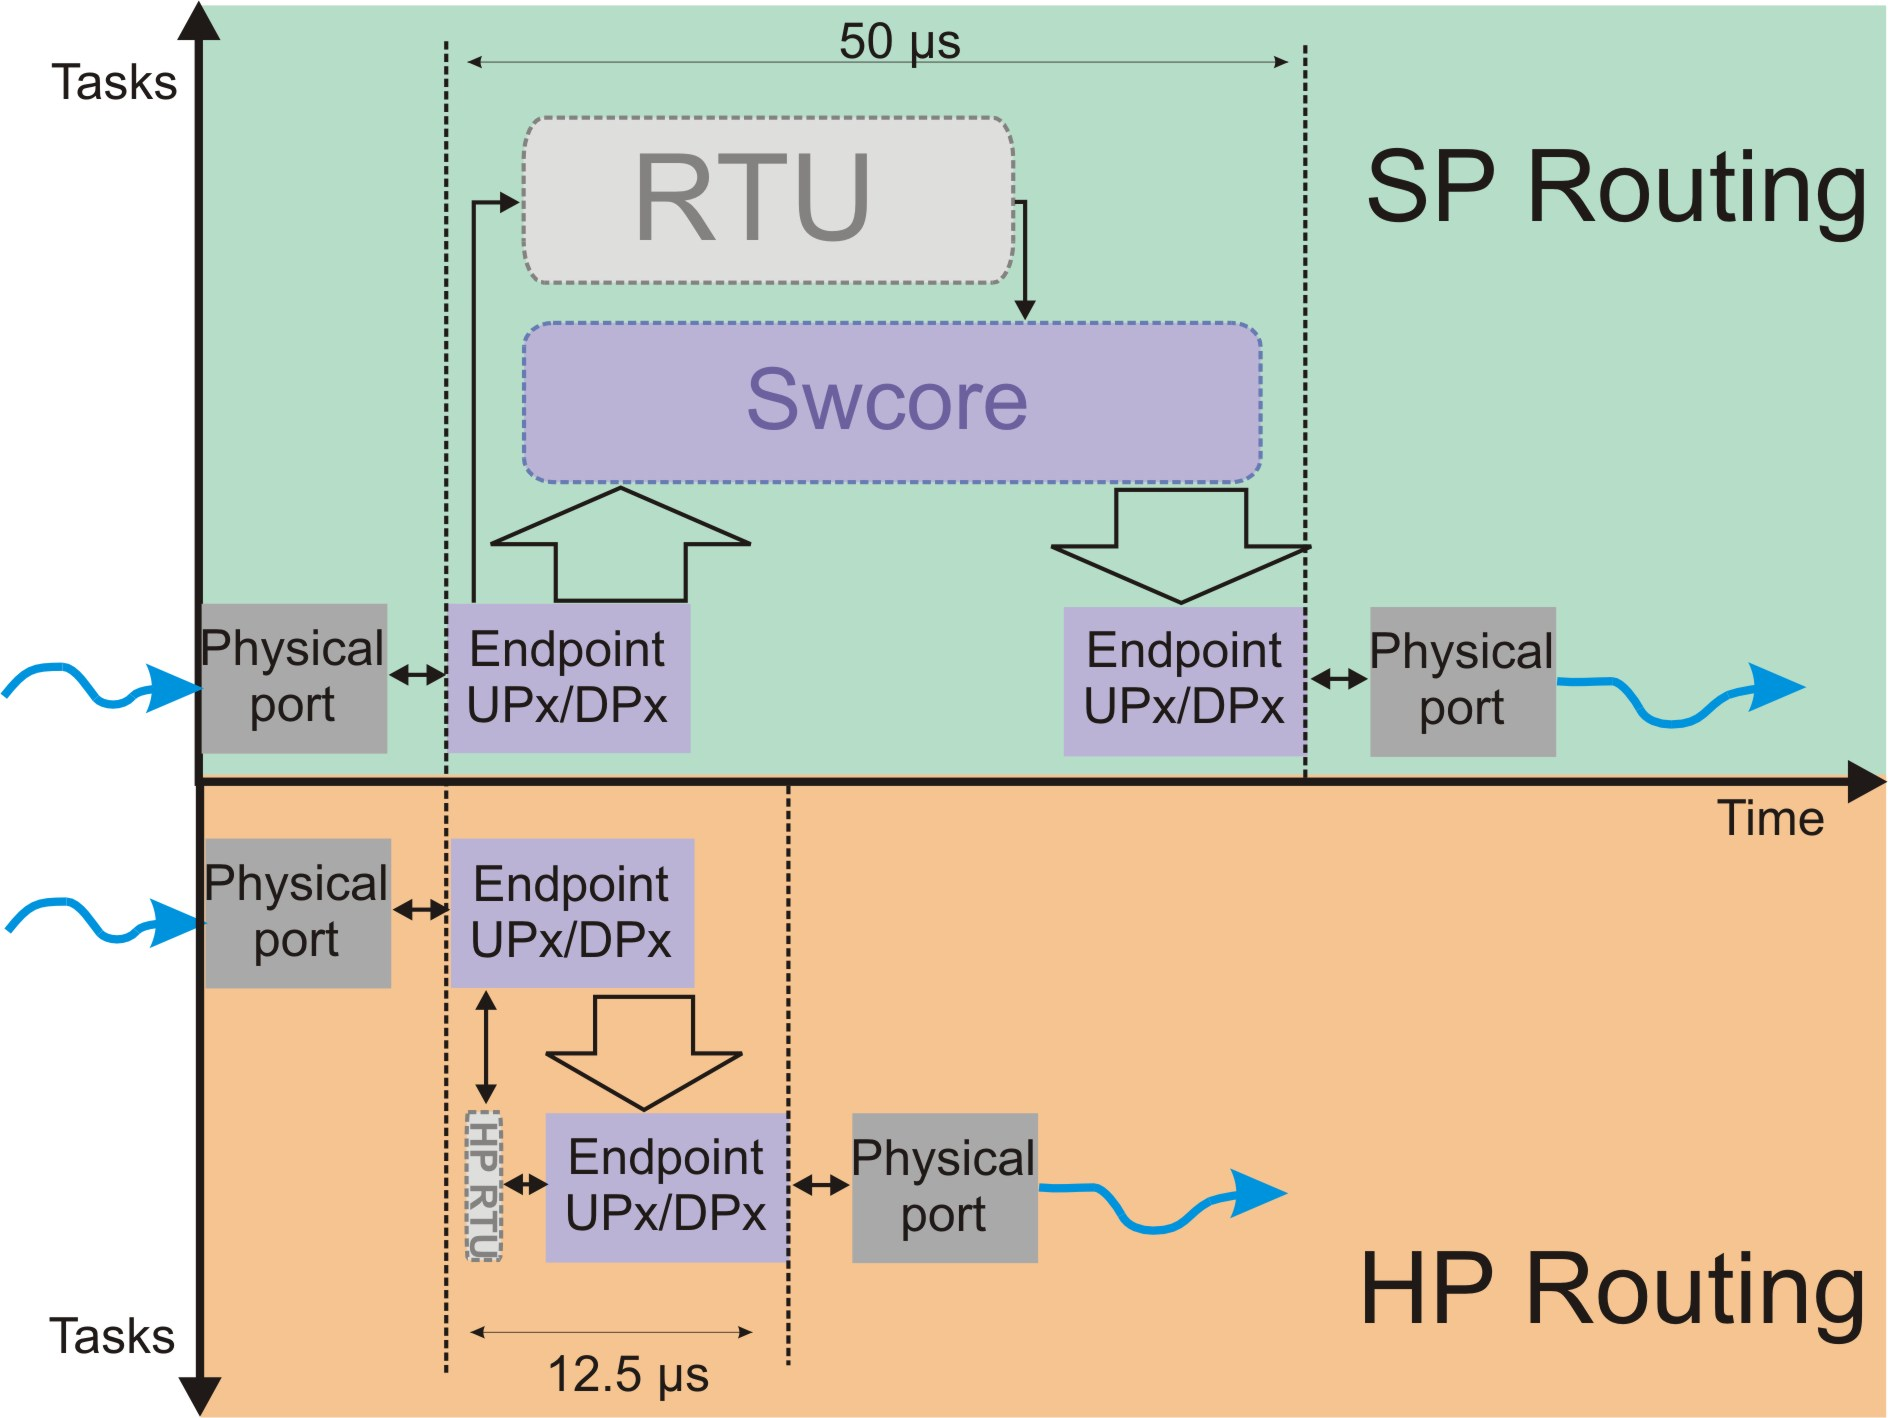
\includegraphics[scale=0.30]{robustness/SWhpRouting.ps}
	\captionof{figure}{Difference between \HP\ and \SP\ Routing (not to
scale).}
	\label{fig:swhprouting}
\end{center}

Due to it's properties, \HP Traffic can be routed separately from \SP\ traffic
in order to increase routing speed, it is called \HighPriority\ Bypass (\HP\
Bypass) in this document. Figure~\ref{fig:swhprouting} ilustrates the difference
between
\SP\ and \HP\ Routing. The following rules for \HP\ Traffic are proposed:
\begin{itemize}
  \item \HP\ Traffic is cut-through routed, if possible.
  \item A \HP\ Package is recognized in the Endpoint as soon as the entire
header has been received.
  \item As soon as a \HP\ Package is recognized, the \HP\ Bypass is stared.
  \item A \HP\ Package is routed according to the settings in the local VLAN
table.
  \item \HP\ Packages coming from the Data Master to the Nodes (down the network
topology) have precedence over the \HP\ Packages travelling up the network
topology (from any Node).
  \item A \HP\ Package waits for the end of the current transmission (no
pre-emption foreseen). 
  \item The active uplink is considered the source of \HP\ Packages coming from
Data Master - \HP\ Packages received on this port are given precedence.
  \item No dropping of \HP\ Packages coming from active uplink is foreseen (in
case of proper functioning) - the buffers should have enough size to ensure
this.
  \item Dropping of \HP\ Packages coming from other ports then active
uplink is foreseen in case of :
  \begin{itemize}
    \item collision with \HP\ Packages coming from active uplinks 
    \item \HP\ Packages burst being already forwarded from other then active
uplink ports.
  \end{itemize}

\end{itemize}


The \HP\ Bypass Algorithm is depicted in Figure~\ref{fig:timePaths}. The
algorithm describes the routing of \HP\ Traffic. \HP\ Package shall be recognized as
soon as its header has been received. It is distinguished by broadcast
destination address and the highest priority (7). \HP\ Traffic is broadcast
within a given VLAN, therefore VLAN port mask needs to be verified for each \HP\
Package. To avoid throughput deterioration due to \HP\ Traffic, the \SP\ Package
is finished sending on the output port on which \HP\ Package is supposed
to be forwarded. This implies having \HP\ output buffer on each port which is
of the size greater or equal to the maximum size of Ethernet Frame. This allows
to store the HP Package while waiting for the \SP\ Package to be sent. It is assumed
that \HP\ Packages received on the active uplink port are sent by the Data
Master, thus they have precedence over \HP\ Packages received from downlink
port.
 
\begin{center}
	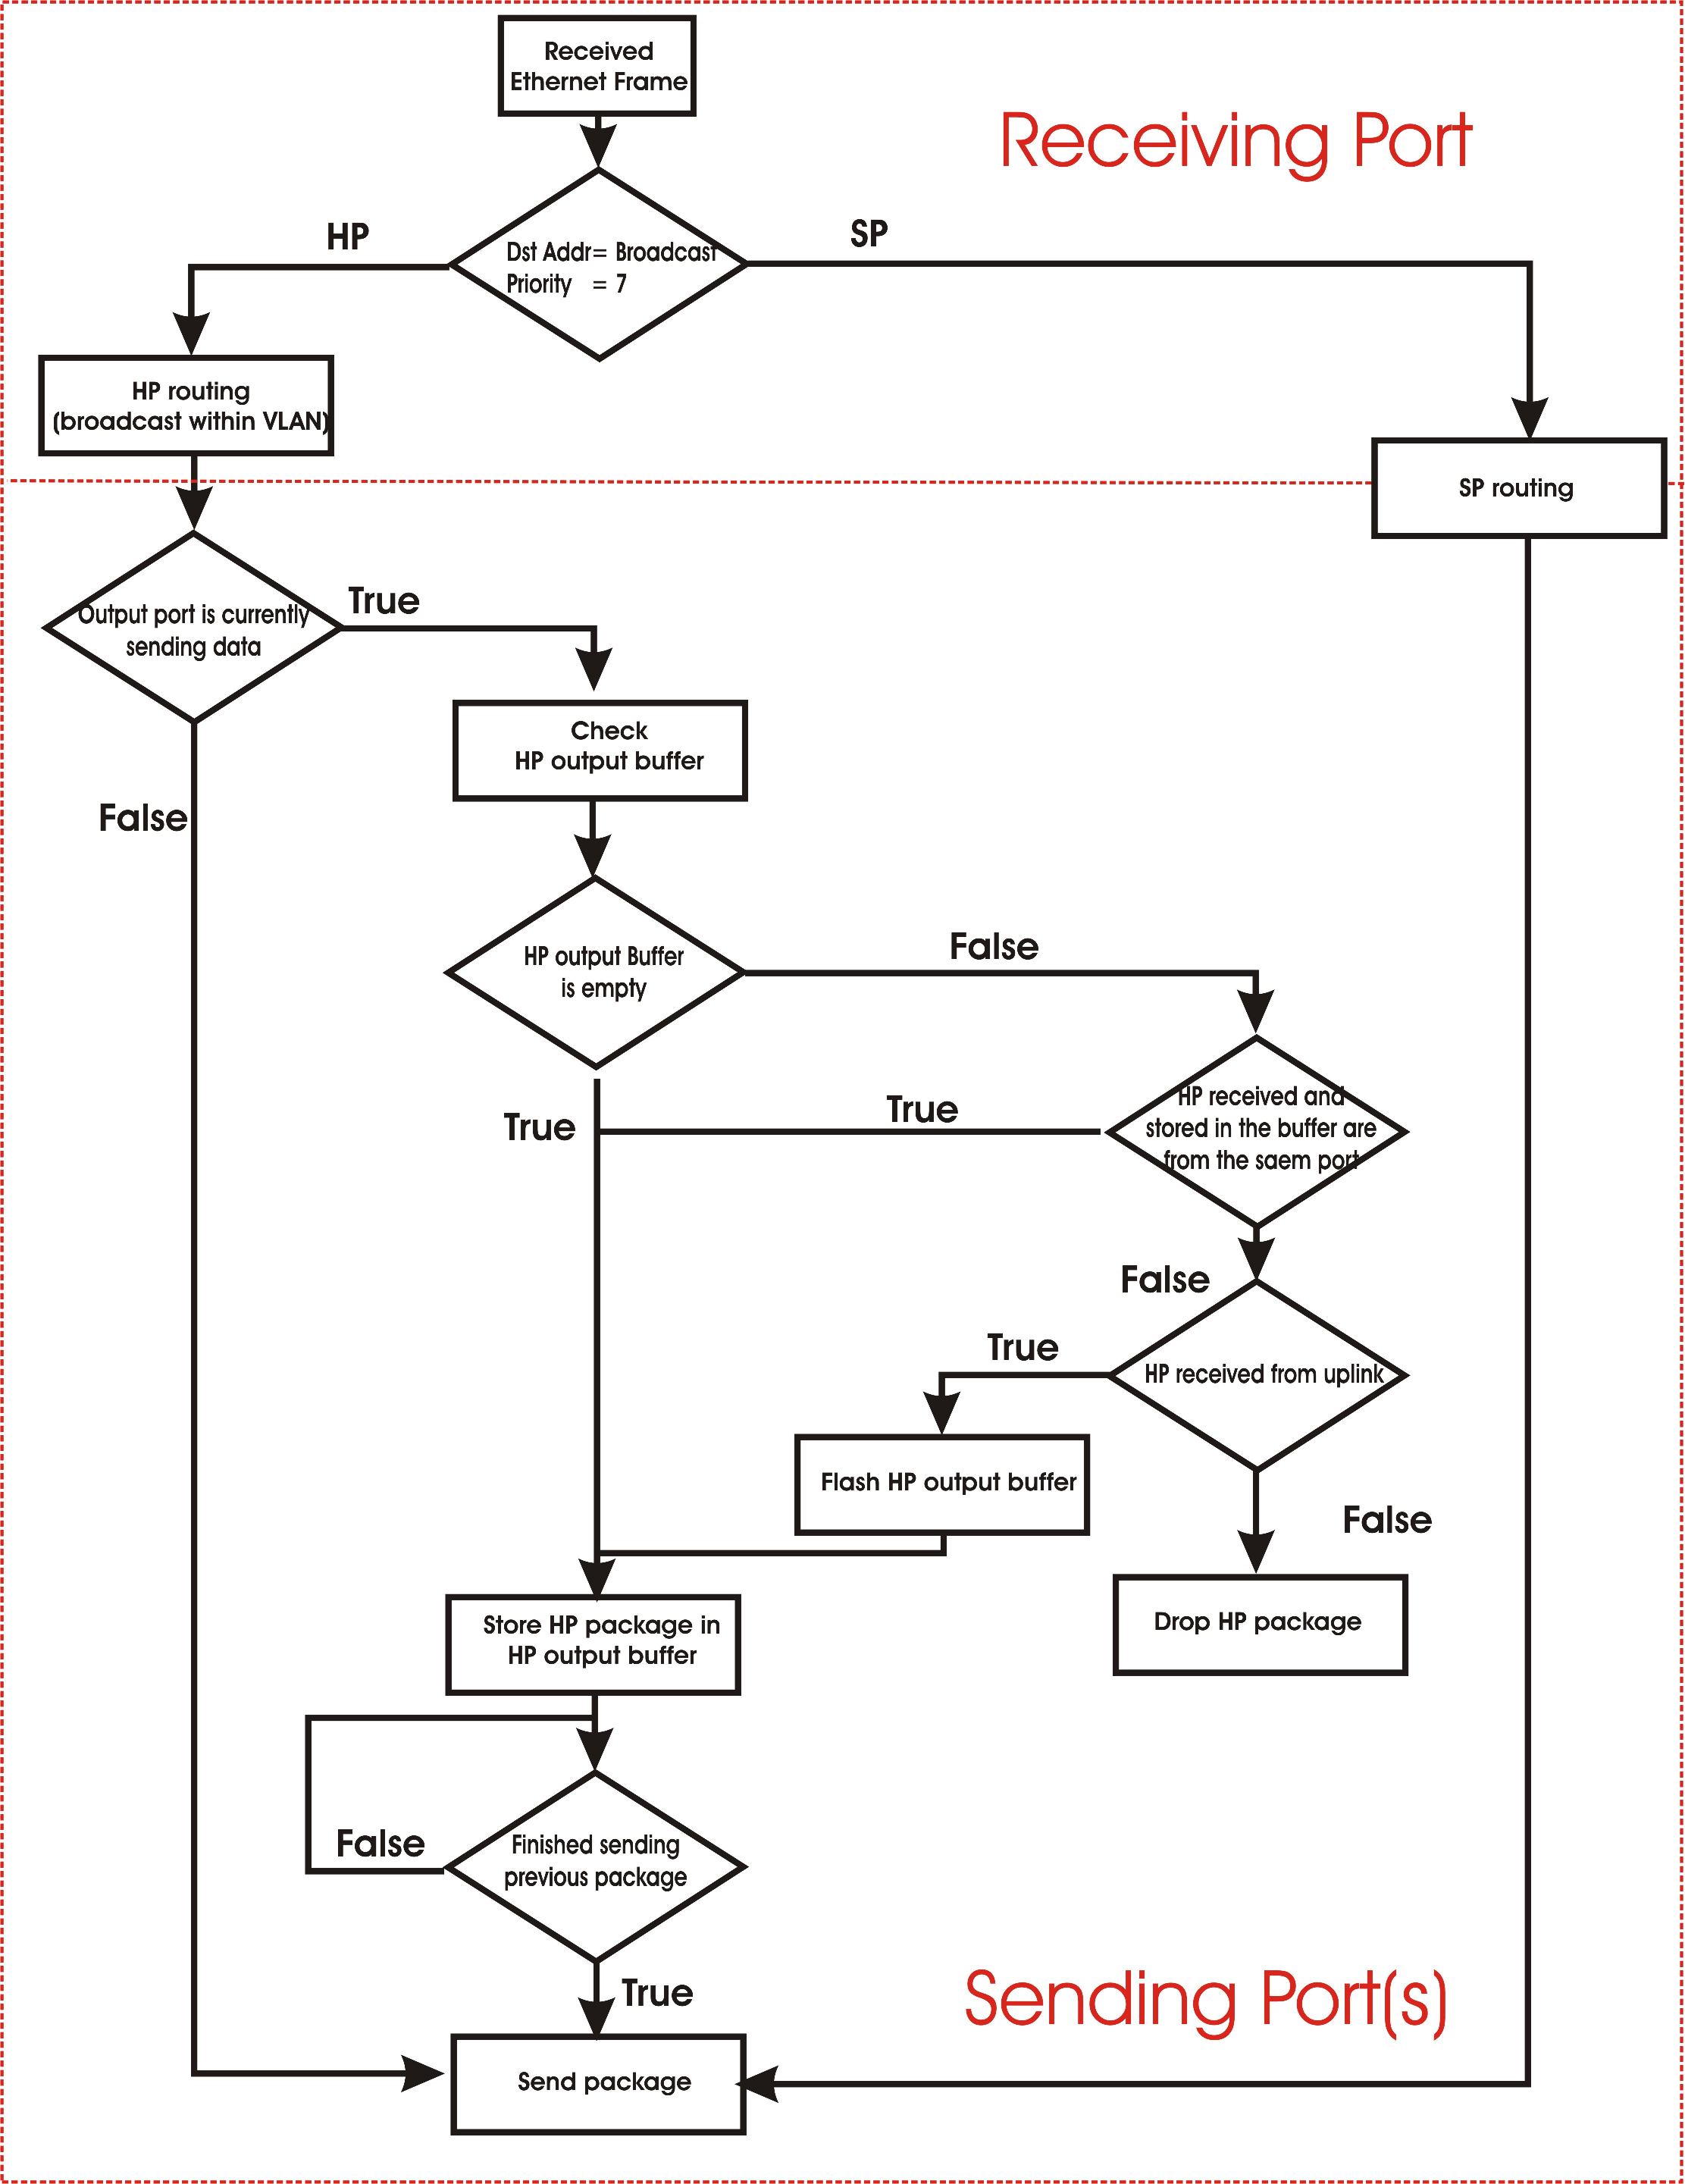
\includegraphics[scale=0.30]{robustness/hpRouting.ps}
	\captionof{figure}{Algorithm for routing \HP\ Traffic.}
	\label{fig:timePaths}
\end{center}


The \HP\ Bypass decreases jitter of \HP\ Traffic routing
on the WR Switch. Table~\ref{tab:CMdelayHP} shows delays of \HP\ Packages on WR
Network components. It can be noted that routing of \HP\ Traffic is considerably
faster. Figure~\ref{fig:CMdelayHP} depicts \ControlMessage\ Delivery Delay
estimation with \HP\ Bypass. For the GSI use case, the CM Delivery Delay
decreased from $221\mu s$ to $78\mu s$, while for CERN scenario the delay
changed from $283\mu s$ to $118\mu s$. Table~\ref{tab:CMspDelay} presents the
estimations for various Control Message sizes.

\begin{table}[ht]
\caption{Control Message Delivery Delay.} 
\centering
	\begin{tabular}{| c | c | c | c |}          \hline
\textbf{Control Message size}& \multicolumn{2}{|c|}{\textbf{\ControlMessage\
Delivery Delay}}\\
               &    GSI           & CERN          \\ \hline
500 bytes      & 78$\mu s$        & 118$\mu s$    \\ \hline
1500 bytes     & 102$\mu s$       & 142$\mu s$    \\ \hline
5000 bytes     & 162$\mu s$       & 202$\mu s$    \\ \hline
\end{tabular}
\label{tab:CMspDelay}
\end{table}


\begin{center}
	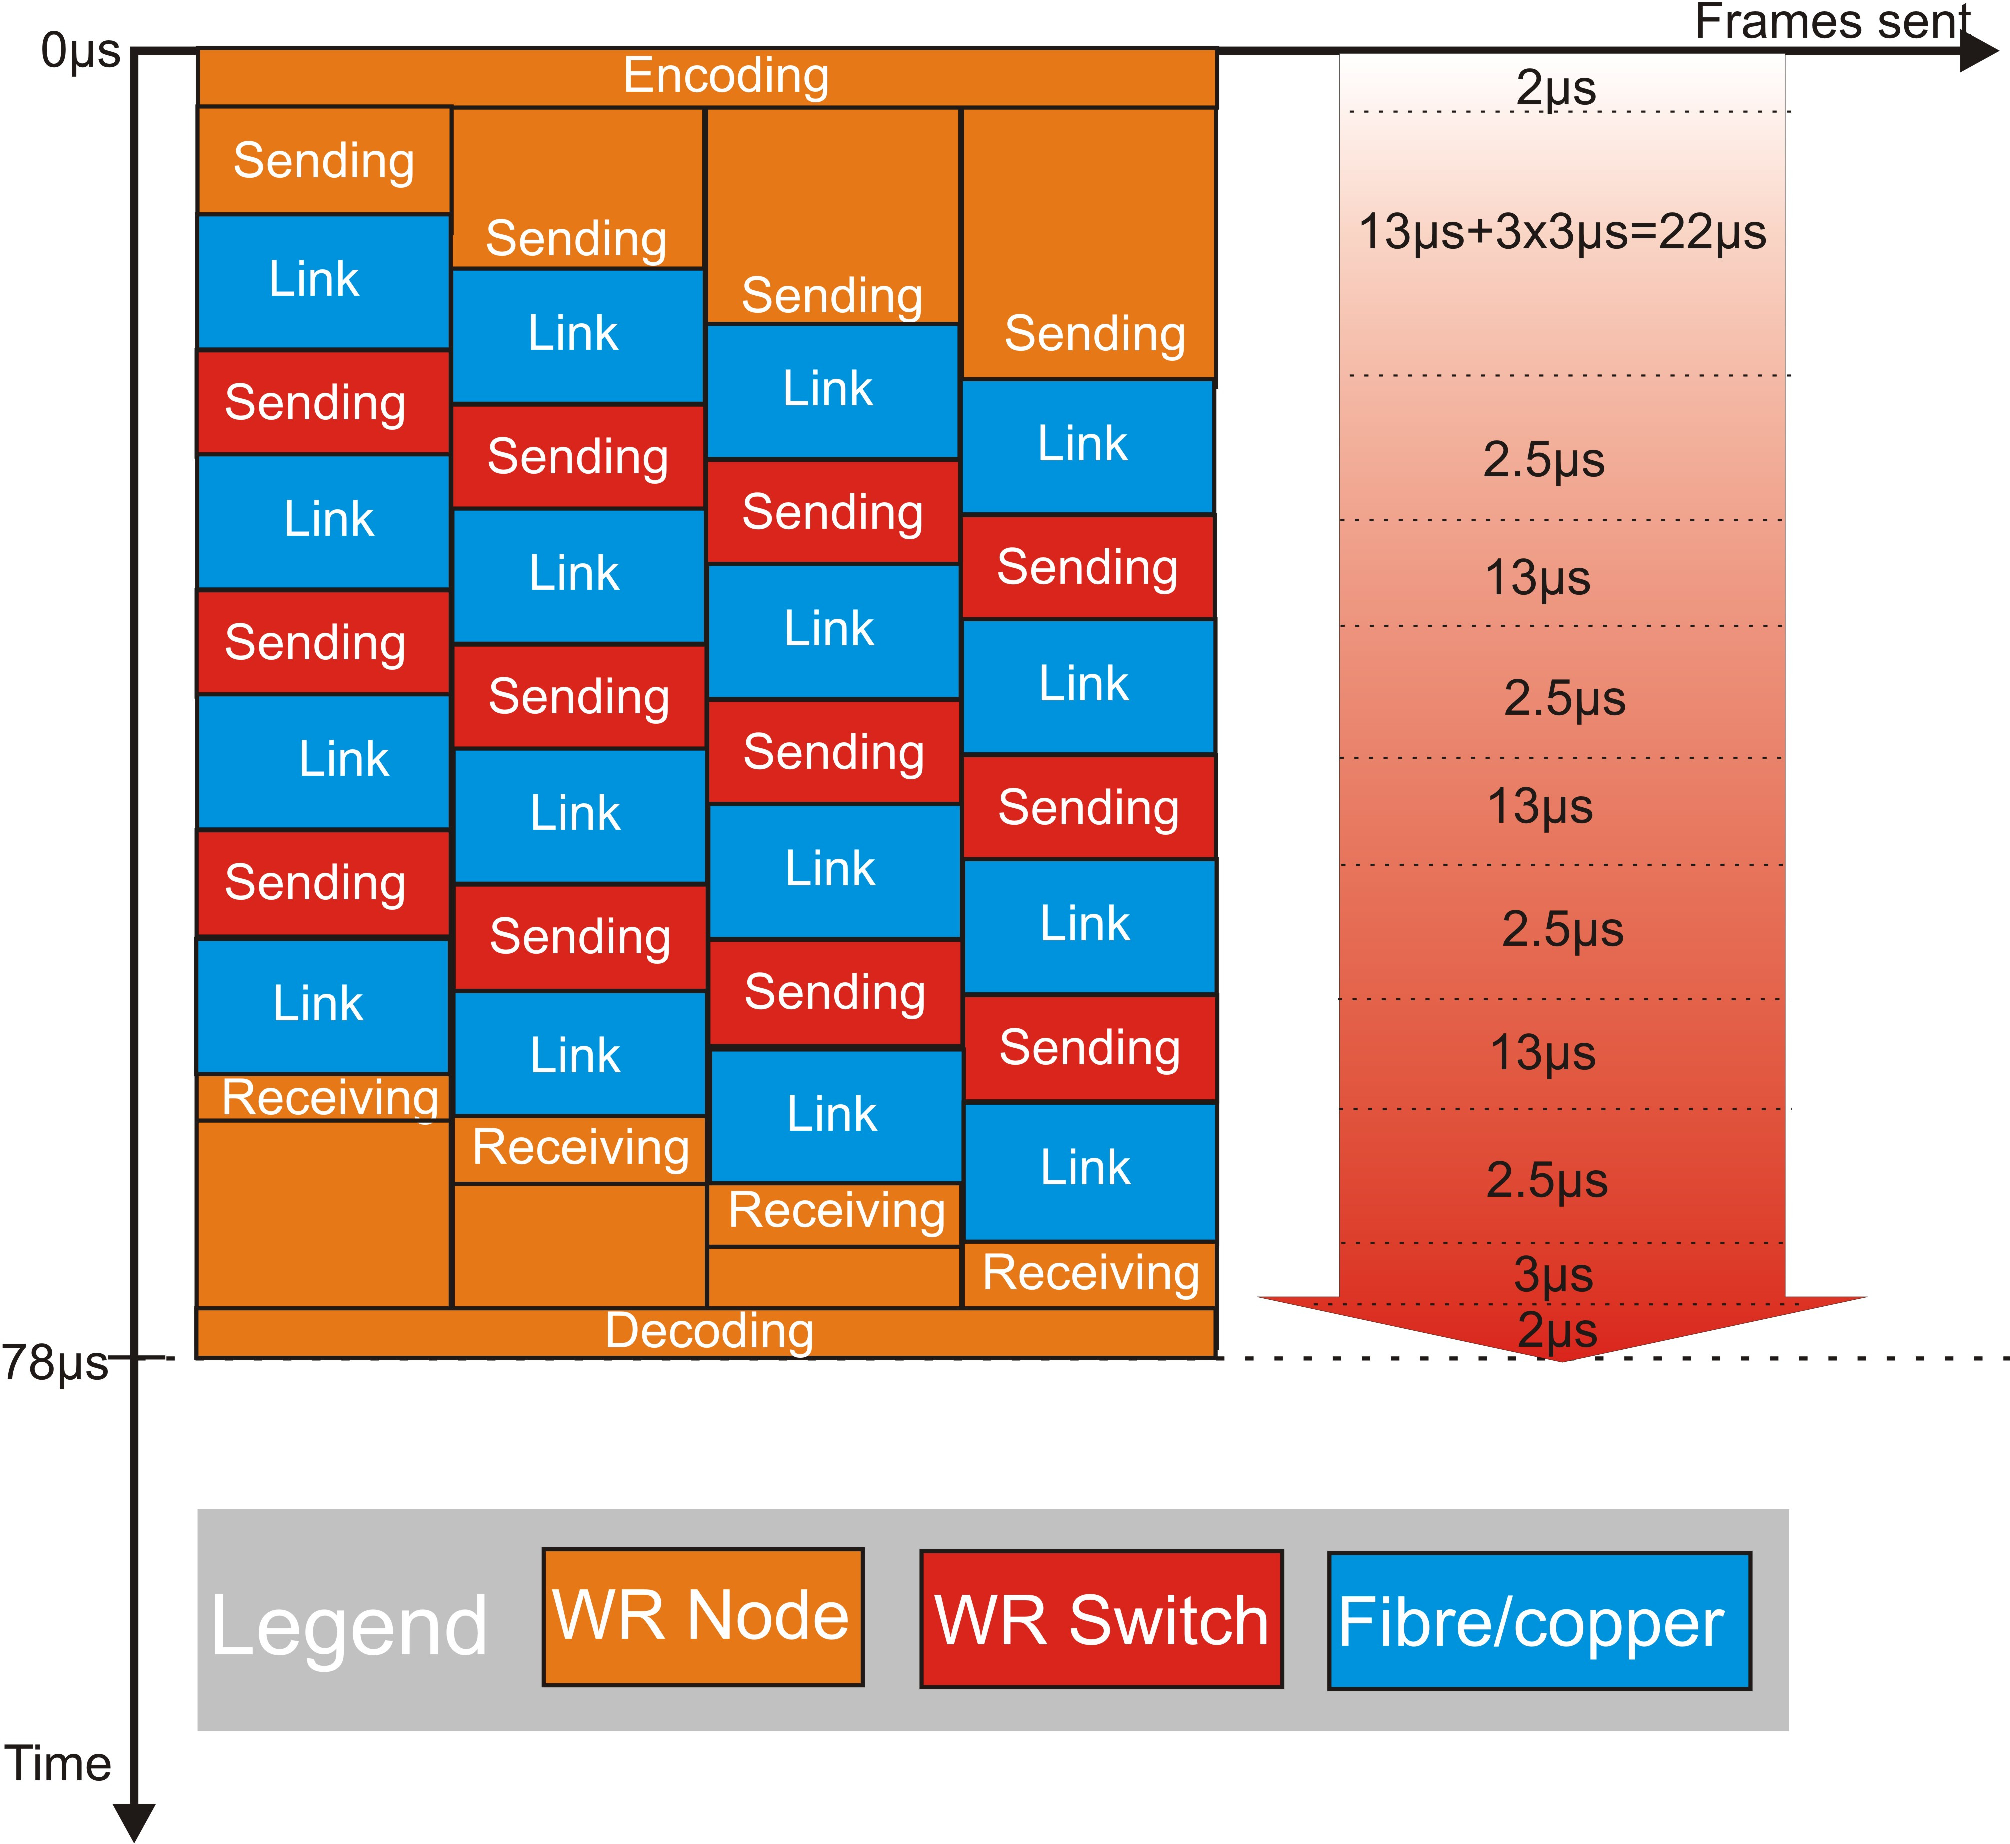
\includegraphics[scale=0.30]{robustness/CMdelayHP.ps}
	\captionof{figure}{Delivery Delay of \ControlMessage\ using \HP\
Bypass.}
	\label{fig:CMdelayHP}
\end{center}

\begin{table}[ht]
\caption{Elements of \ControlMessage\ frame delivery delay estimation.} 
\centering
	\begin{tabular}{| l |  c | c | c |}          \hline
\textbf{Name}&\textbf{Symbol}&\textbf{Value}&\textbf{Value}                  \\
                                 &                &  Min& Max          \\ \hline
% Sending node
Ethernet Frame Transmission Delay&$delay_{n\_tx}$&$0\mu s$&$(13 + B_{tx}
*t_{FECpck})
\mu s$
\\ \hline
% Switch
Switch Routing Delay            &$delay_{n\_sw}$&$~0\mu s$&$13\mu s$ 
 
\\ \hline
% Links
Link Delay                       & $delay_{link}$ &5 [$\frac{\mu
s}{km}$]&5 [$\frac{\mu s}{km}$]      
\\ \hline
% Receivning node
Ethernet Frame Reception delay   & $delay_{n\_rx}$&$t_{FECpck}\mu
s$&$t_{FECpck}\mu s$
\\ \hline
%encoding
FEC Encoding                     & $delay_{enFEC}$&$2\mu s$&$2\mu s$
\\ \hline
%decoding
FEC Decoding                     & $delay_{deFEC}$&$2\mu s$&$2\mu s$
\\ \hline

\end{tabular}
\label{tab:CMdelayHP}
\end{table}

$t_{FECpck} = \{3,9,12\} \mu s$ for 500, 1500 and 5000 bytes size
\ControlMessage s respectively.
$B_{tx} = {3,3,7}$ for for 500, 1500 and 5000 bytes size \ControlMessage s
respectively.
 
